\begin{explanationbox}
\textbf{\textcolor{CExplanation}{为什么会想到这个结论？}}\par
一道题说“两个根都在$(m,n)$内”。直接解根式常常很麻烦，尤其系数含参数。换个角度：\textbf{根就是抛物线与$x$轴的交点}，只看图就能把要求变成几个简单不等式。

\medskip
\textbf{\textcolor{CExplanation}{第一眼：$\Delta$只告诉你有没有交点}}\par
例如$f(x)=x^2-1$有两个交点$-1,1$，但是$(2,3)$内一个也没有。\textbf{$\Delta>0$只保证“有两个”，不保证“都在指定区间”。}
\begin{center}
\begin{tikzpicture}[x=.95cm,y=.68cm,>=stealth]
 \draw[->] (-1.8,0)--(3.55,0) node[right]{$x$};\draw[->] (0,-1.5)--(0,3.0) node[above]{$y$};
 \draw[very thick,blue!75!black,domain=-1.65:1.85,samples=65] plot (\x,{\x*\x-1});
 \draw[line width=1.5pt,green!55!black] (2,0)--(3,0);
 \draw[fill=white,green!60!black] (2,0) circle (2pt) (3,0) circle (2pt);
 \fill[red] (-1,0) circle (1.8pt) (1,0) circle (1.8pt);
 \node[below] at (-1,0) {$-1$};\node[below] at (1,0) {$1$};
 \node[below] at (2,0) {$2$};\node[below] at (3,0) {$3$};
 \node[above,green!45!black] at (2.5,.1) {所求区间};
\end{tikzpicture}

\end{center}

\textbf{\textcolor{CExplanation}{第二眼：对称轴为什么要在区间中间？}}\par
两个不同根$x_1<x_2$左右对称，对称轴$x_0=\frac{x_1+x_2}{2}$恰好在两根中间。若两个根都在$(m,n)$，一定有$m<x_0<n$。\textbf{但只有对称轴在区间内仍不够：两根可能离得太远！}

\medskip
\textbf{\textcolor{CExplanation}{第三眼：为什么看$af(m)$、$af(n)$？}}\par
开口向上的抛物线在两根\textbf{外侧为正}；开口向下时在两根\textbf{外侧为负}。所以两端点若都在根的外侧，端点函数值总与$a$同号：$af(m)>0,af(n)>0$。
\begin{center}
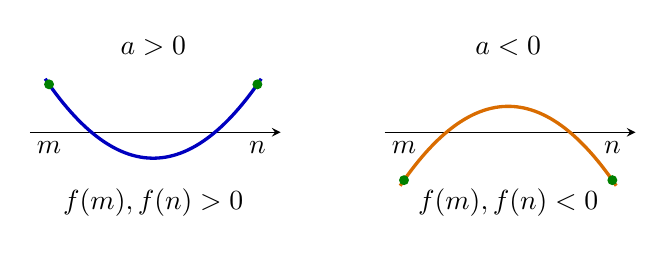
\begin{tikzpicture}[x=.98cm,y=.83cm,>=stealth]
 \begin{scope}[shift={(-2.3,0)}]
  \draw[->] (-1.6,0)--(1.65,0);\draw[very thick,blue!75!black,domain=-1.4:1.4,samples=60] plot (\x,{.62*(\x*\x-.64)});
  \node[above] at (0,1.02) {$a>0$};\node[below] at (-1.35,0) {$m$};\node[below] at (1.35,0) {$n$};
  \fill[green!50!black] (-1.35,{.62*(1.35*1.35-.64)}) circle(1.8pt) (1.35,{.62*(1.35*1.35-.64)}) circle(1.8pt);
  \node[below] at (0,-.72) {$f(m),f(n)>0$};
 \end{scope}
 \begin{scope}[shift={(2.3,0)}]
  \draw[->] (-1.6,0)--(1.65,0);\draw[very thick,orange!85!black,domain=-1.4:1.4,samples=60] plot (\x,{-.62*(\x*\x-.64)});
  \node[above] at (0,1.02) {$a<0$};\node[below] at (-1.35,0) {$m$};\node[below] at (1.35,0) {$n$};
  \fill[green!50!black] (-1.35,{-.62*(1.35*1.35-.64)}) circle(1.8pt) (1.35,{-.62*(1.35*1.35-.64)}) circle(1.8pt);
  \node[below] at (0,-.72) {$f(m),f(n)<0$};
 \end{scope}
\end{tikzpicture}

\end{center}
\textbf{一个眼前一亮的简化：}$a$不论正负，$a^2>0$。又因$f(m)=a(m-x_1)(m-x_2)$，所以$af(m)=a^2(m-x_1)(m-x_2)$。\textbf{这样一来，判断端点在两根外侧就不必单独分开口方向了。}

\medskip
\textbf{\textcolor{CExplanation}{一个根时为什么不能只背“异号”？}}\par
端点异号说明从一端走到另一端，图像穿过$x$轴\textbf{奇数次}；二次函数最多有两个不同根，因此只能穿过一次。但图像在区间内部\textbf{刚好碰到}轴后又回去（重根）时，两端可能同号；若某个根就在被排除的端点上，乘积又会等于$0$。
\begin{center}
\begin{tikzpicture}[x=1cm,y=.75cm,>=stealth]
 \begin{scope}[shift={(-2.45,0)}]
  \draw[->] (-1.35,0)--(1.4,0);
  \draw[very thick,blue!70!black,domain=-1.15:1.15,samples=55] plot (\x,{.65*\x*\x});
  \draw[dashed,gray] (0,0)--(0,1.05);\fill[red] (0,0) circle(1.7pt);
  \node[below] at (-1.15,0) {$m$};\node[below] at (1.15,0) {$n$};
  \node[above] at (0,1.1) {相切：重根};
 \end{scope}
 \begin{scope}[shift={(2.15,0)}]
  \draw[->] (-1.35,0)--(1.45,0);
  \draw[very thick,orange!80!black,domain=-1.1:1.2,samples=55] plot (\x,{.65*(\x+.8)*(\x-.3)});
  \fill[red] (-.8,0) circle(1.7pt) (.3,0) circle(1.7pt);
  \node[below] at (-.8,0) {$m$};\node[below] at (.3,0) {$x_2$};\node[below] at (1.2,0) {$n$};
  \node[above] at (0,1.1) {端点也是根};
 \end{scope}
\end{tikzpicture}

\end{center}

\textbf{\textcolor{CExplanation}{考试什么时候用最快？}}\par
遇到“含参数二次方程的根在某个区间内”，先画很小的草图，再列$\Delta$、对称轴、两端符号；若只问一个根，先查两端异号，\textbf{不异号时再排查重根和端点根}，避免漏掉边界。
\end{explanationbox}
